%!TEX root = ../Thesis.tex

\chapter{Interpretation of Boxplots}\label{app: Appendix: Boxplot interpretation}

\begin{figure}[H]
    \centering
    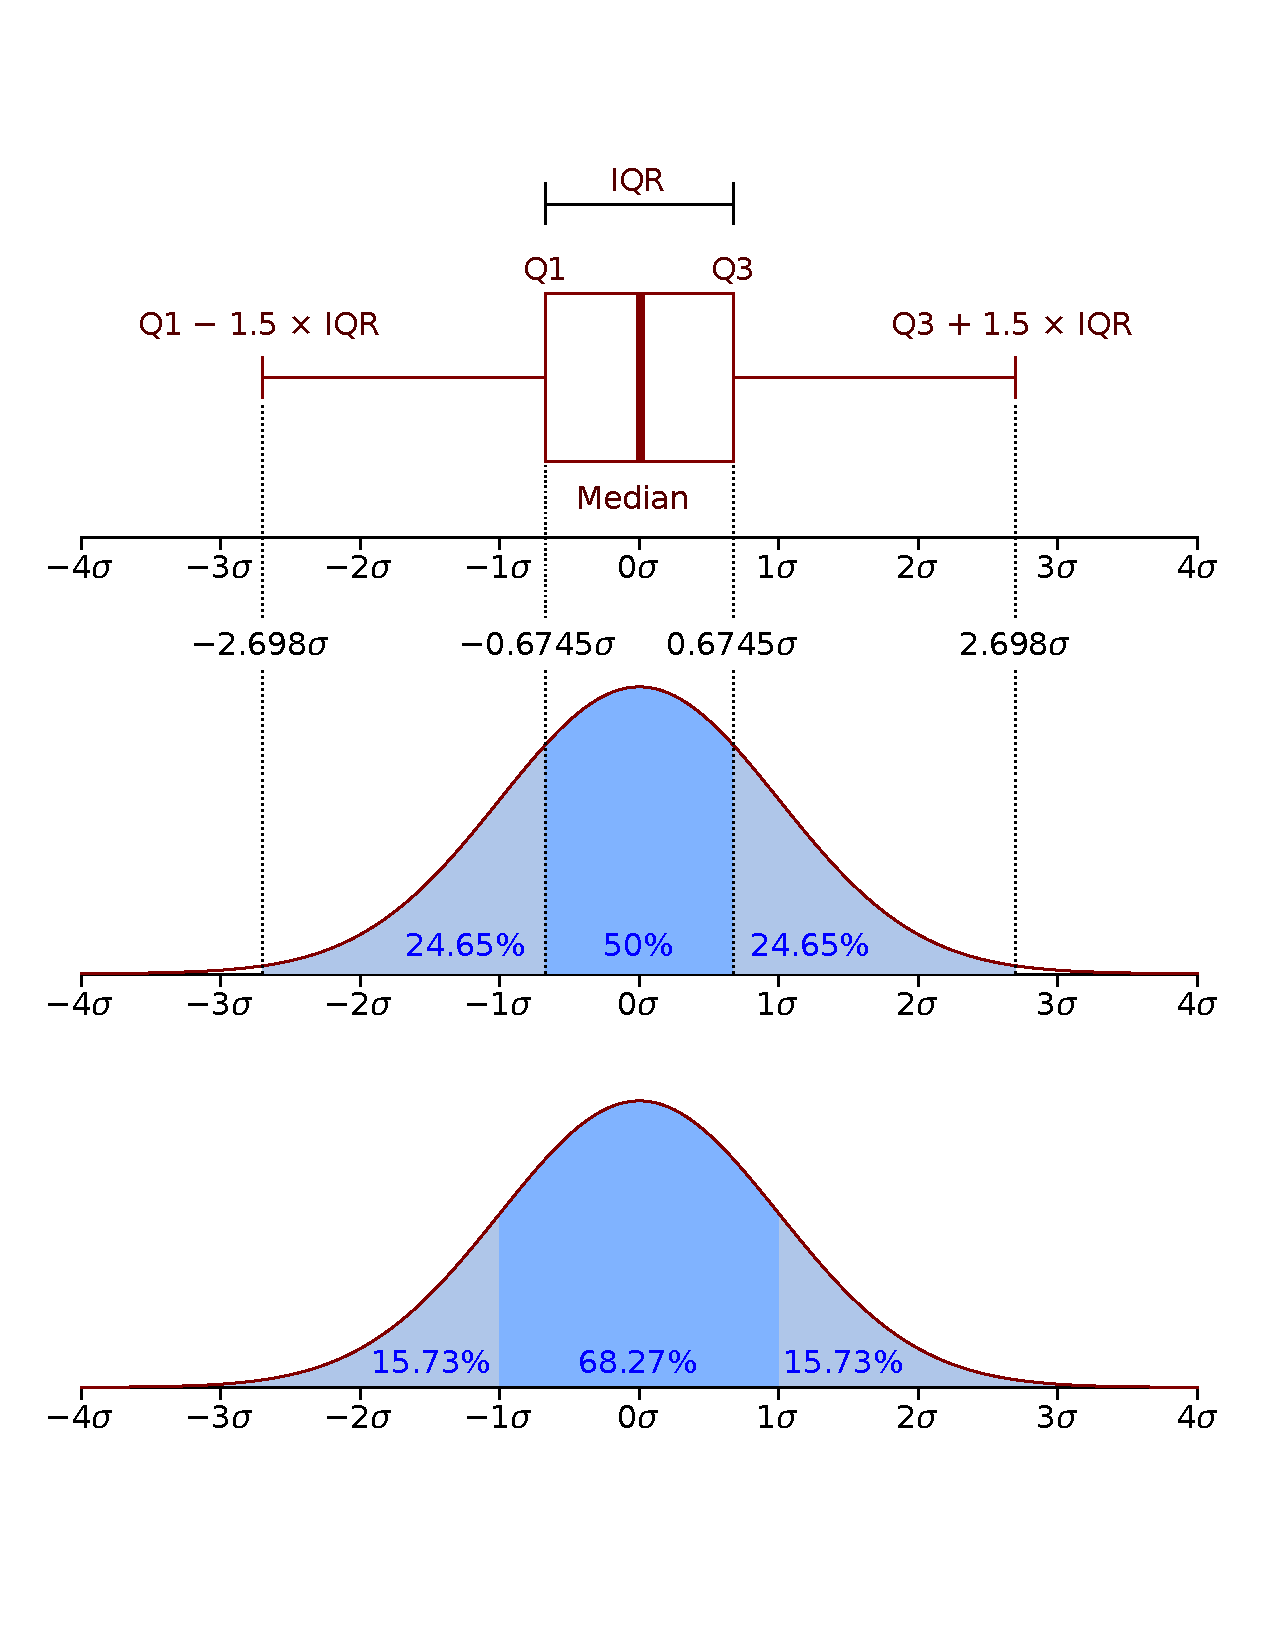
\includegraphics[width=0.8\textwidth]{graphics/boxplot/Boxplot_vs_PDF.pdf}
    \caption{
        Interpretation of boxplots. This figures illustrates how to interpret the boxplots shown in this thesis. Note that the median, first and second quartiles and the interquartile range (IQR) are defined in relation to the boxplot and put into the perspective of normally distributed data. Obviously, not all data is normal which can for instance result in non-symmetric boxplots. Figure due to \url{https://en.wikipedia.org/wiki/Interquartile_range}.
    }
    \label{fig: Appendix: boxplot interpretation}
\end{figure}
